\documentclass[10pt]{beamer}

%%%
% PREAMBLE FOR THIS DOC 
%%%
%https://tex.stackexchange.com/questions/68821/is-it-possible-to-create-a-latex-preamble-header
\usepackage{/Users/miw267/Repos/latex_preamble/beamer_preamble}





%%%
% AGENDA TOPICS
%%%
\agendatopic[quiz]{Quiz Updates}
\agendatopic[review]{Review of Counterexamples}
\agendatopic[boolean]{Boolean Algebra}


%%%
% DOCUMENT
%%%

\begin{document}

%\maketitle

%% Title page frame
%\begin{frame}
%    \titlepage 
%\end{frame}





\title{09/09/2025: Boolean Algebra}
\author{CSCI 246: Discrete Structures}
\date{Textbook reference: Sec. 7, Scheinerman}

\begin{frame}
    \titlepage 
\end{frame}




\begin{frame}

\vfill 
\begin{mygreenbox}[title=Quiz return method]
Quizzes are grouped into four bins (A-G, H-L, M-R, S-Z) by last name. \\
The quizzes are upside down with your last name on the back. \\
Come find yours before, during, or after class. \\
Only turn the quiz over if it's yours.
\end{mygreenbox} 
\vfill 

\begin{myyellowbox}[title=Today's Agenda]
\begin{itemize}
	\item Quiz updates ($\approx$ 5 mins)
	\item Review counterexamples ($\approx$ 15 mins)
	\item Boolean algebra ($\approx$ 15 mins)
	\item Group exercises ($\approx$ 15 mins)
\end{itemize}

\end{myyellowbox}
\end{frame}




\agendaframe{quiz}



\begin{frame}{Weekly Quiz \#1: Scores}

\begin{figure}[ht]
        \centering
        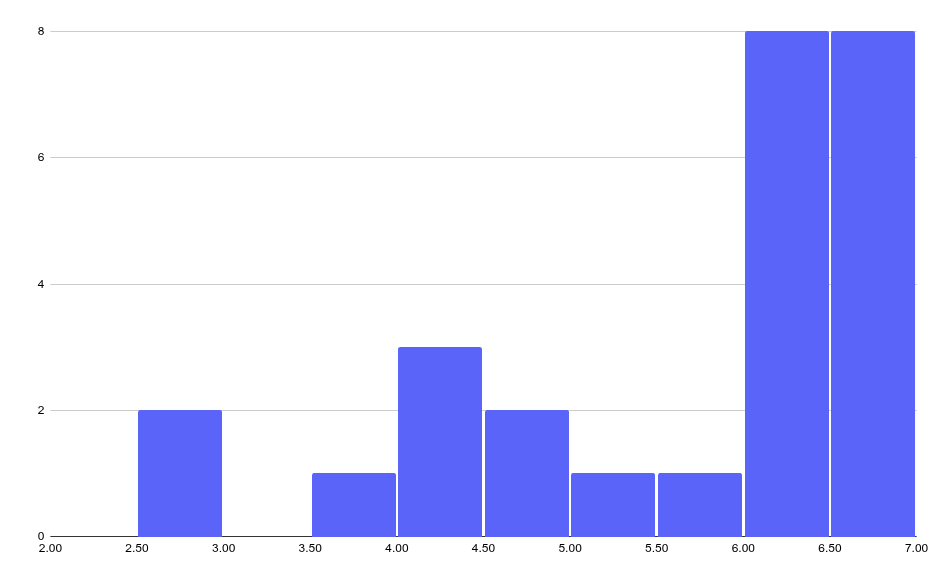
\includegraphics[width=\textwidth]{images/quiz1_scores}
        \caption{Reading Quiz Scores. Median: 6/7 (85.7\%). See repo for feedback.}
\end{figure}
\vfill 

\end{frame}


%\begin{frame}{Review of Weekly Quiz \#1}
%
%\begin{myredbox}[title=Reflections ($\approx$ 3 min)]
%Take out a sheet of paper and tell me about your experience with the quiz -- How was it? \\
%
%In particular, I'm interested in:
%\begin{enumerate}
%\item What can you do to help prepare yourself for future quizzes?	
%\item What can I do to help prepare you for future quizzes?
%\end{enumerate}
%\end{myredbox}
%			
%\end{frame}


\begin{frame}{Study Guide For Quiz 2}


\begin{myredbox}[title=Readings (1 question)]
Sec 5 (Proofs)
\begin{itemize}
\item Know how to prove Props 5.2, 5.3, 5.5, and 5.6.
\end{itemize}
Sec. 6 (Counterexample)
\begin{itemize}
\item Know how to apply Proof Template 3.
\item In particular, know how to disprove Statement 6.1. 
\end{itemize}
%Sec. 7 (Boolean Algebra)
%\begin{itemize}
%\item Know how to prove Props 7.1 and 7.3 using truth tables.
%\item Understand the Boolean algebra properties listed in Theorem 7.2.  (What are they saying? Could you imagine proving them using truth tables?)
%\end{itemize}

\end{myredbox}

\vfill 

\begin{myyellowbox}[title=Group exercises (2 questions)]
Know how to do all of the group exercises from these 2 sections.
\end{myyellowbox}

\end{frame}




\agendaframe{review}


\begin{frame}{Review of Sec. 6 (Counterexamples)}
\label{frame:assumption_not_met}
\footnotesize  
 \begin{mybluebox}
Disprove the following conjecture:  
\textit{Let $a$ and $b$ be integers.  If $a|b$ and $b|a$, then $a=b$.}  
\end{mybluebox}
\vfill 

\only<2->{
\begin{myyellowbox}[title=Poll]
Is $a=1, b=0$ a valid counterexample?
\end{myyellowbox}
}

\vfill 

\only<3-4>{
\colorbox{blue!30}{\textbf{Recall.}} Here's the truth table for unidirectional implication.
\begin{center}
\begin{tikzpicture}
\node[inner sep=0pt] (tbl) {%
\renewcommand{\arraystretch}{1.35}%
\begin{tabular}{cc|c}
\alert{X} & \alert{Y} & $\overbrace{\alert{X} \implies \alert{Y}}^{\text{If \alert{X}, then \alert{Y}}}$ \\
\hline
T & T & \green{T} \\
T & F & \red{F} \\
F & T & \green{T}  \\
F & F & \green{T}  \\
\end{tabular}};
\only<2->{%
  \draw[black, line width=2pt] ([yshift=-0.23cm]tbl.center) ellipse (1.9cm and 0.32cm);
  \node[anchor=west, font=\Large] (lbl) at (2.65,-0.23) {counterexamples live here};
  \draw[black, line width=1.2pt, ->] (lbl.west) -- ++(-0.6,0);
}
\end{tikzpicture}
\end{center}
}

\only<4>{
\colorbox{green!30}{\textbf{Interpretation.}}
So we need to find a case where proposition $X=\set{a|b \text{ and } b|a}$ is true but proposition $Y=\set{a=b}$ is false.
}

\only<5->{
	\begin{mydef}[title=Reminder of Definition 3.2 (\textbf{Divisible})]
	Let $a$ and $b$ be integers.  We say that $a$ is \textit{divisible} by $b$ provided there is an integer $c$ such that $bc=a$. The notation for this is $b|a$. 
	\end{mydef}
}
\vfill 	

\only<6->{
\footnotesize 
\textbf{Solution to poll:} The proposition $\red{a}|\blue{b} \; (= \red{1}|
\blue{0})$ is \texttt{true}, since there is an integer $\green{c}$ (namely $\green{c=0}$) such that $\red{a}\green{c}=\blue{b}$ (since $\red{1} \cdot \green{0} = \blue{0}$). However, the proposition $\blue{b}|\red{a} \; (= \blue{0}|\red{1})$ is \texttt{false}, since there is no integer $\purple{d}$ such that $\blue{b}\purple{d}=\red{a}$ (that is, there is no integer $\purple{d}$ such that  $\blue{0}\cdot \purple{d} = \red{1}$). Overall, \alert{the hypothesis doesn't hold, so we have not disproven the statement}.  
}
\end{frame}


\begin{frame}{Review of Sec. 6 (Counterexamples)}
\footnotesize 

 \begin{mygreenbox}
\footnotesize 
Disprove the following conjecture: \textit{Let $a$ and $b$ be integers.  If $a|b$ and $b|a$, then $a=b$.}
\end{mygreenbox}

\vfill 
\begin{myyellowbox}
Is $a=5, b=-5$ a valid counterexample? \pause  Yes it is!  See the proof below.
\end{myyellowbox}
\vfill 

\vfill \vfill 
\footnotesize 

\begin{tabularx}{\textwidth}{L{3cm}X}
\onslide*<3->{\textbf{Annotation} & \textbf{Main Text}} \\
\onslide*<4->{\hlorange{High-level structure} & \hlorange{Let $a=5$, $b=-5$. First, we show that the hypothesis holds [i.e., that $(5|-5)$ and $(-5|5)$].}} \\
\onslide*<5->{\hlgreen{Unravel defn.} & \hlgreen{$a|b$ means there is an integer $x$ such that $ax=b$. Likewise $b|a$ means there is an integer $y$ such that $by=a$.}} \\
\onslide*<6->{\hlred{The ``Glue"} & \hlred{Substituting for $a$ and $b$, we need to show that there are integers $x$ and $y$ such that $5x=-5$ and $-5y=5$.   We see these equations hold by taking $x=-1$ and $y=-1$.}} \\
\onslide*<7->{\hlorange{High-level structure}  & \hlorange{Hence $5|-5$ and $-5|5$, so the hypothesis is met.}} \\
\onslide*<8->{\hlorange{High-level structure}  & \hlorange{Now we show that the conclusion fails [i.e. that $-5\neq5$.]}} \\
\onslide*<9->{\hlred{The ``Glue"} &  \hlred{This is immediately clear.}} \\
\end{tabularx}

\end{frame}



\begin{frame}{Review: how to give a counterexample}

\begin{mygreenbox}[title=Unidirectional implication: $\red{X} \implies \blue{Y}$]
Exhibit \textbf{one} case in which
\begin{itemize}
	\item the hypothesis \red{$X$} \textbf{holds}, and
	\item the conclusion \blue{$Y$} \textbf{fails}.
\end{itemize}
\vspace{0.2em}
To check either one, you must \alert{unravel the definitions} inside \red{$X$} and \blue{$Y$}.
\end{mygreenbox}

\vfill
\pause

\begin{myyellowbox}[title=Poll]
What do you have to show to give a counterexample to a bidirectional implication:  a proposition of the form $X \iff Y$?
\end{myyellowbox}

\vfill
\pause

\begin{myredbox}[title=Solution]
Show that \alert{\textbf{either}} direction fails: \textbf{either} that
$X \implies Y$ fails, \textbf{or} that $Y \implies X$ fails.
%\vspace{0.2em}

%One broken direction is enough.  
%You do \textbf{not} need both.
\end{myredbox}

\end{frame}

\begin{frame}{A note}

\begin{myyellowbox}[title=Poll]
Is the following statement true or false? 
\[ -5|5 = -1 \] 
\end{myyellowbox}

\pause 

\begin{myredbox}[title=Alert!]
In mathematical reasoning, you always need to \textbf{refer back to the definitions}.    
\end{myredbox}

\pause 
	\begin{mydef}[title=Reminder of Definition 3.2 (\textbf{Divisible})]
	Let $a$ and $b$ be integers.  We say that $a$ is \textit{divisible} by $b$ provided there is an integer $c$ such that $bc=a$. The notation for this is $b|a$. 
	\end{mydef}
\pause 
\footnotesize 
Solution to poll: The statement is \textbf{incorrect}! Why? \pause $-5|5$ is a \textbf{proposition}, so it can't equal $-1$. We would instead write just $-5|5$, or perhaps $-5|5 = \texttt{TRUE}$. %How do we justify the proposition? \pause We have $-5|5$ because if $a=5$ and $b=-5$, there exists an integer (namely $c=-1$) such that $bc=a$.
\end{frame}










\agendaframe{boolean}


\begin{frame}{Boolean algebra}

\begin{myyellowbox}[title=What is algebra?]
\textbf{Algebra} lets us reason about \alert{numbers}.  For example, using algebra, we can show that
\[ x^2 - y^2 = (x-y)(x+y) \]	
\end{myyellowbox}


\vfill 
\pause 

\begin{mygreenbox}[title=What is Boolean algebra?]
\textbf{Boolean Algebra} lets us reason about \alert{propositions}.   For instance, using Boolean Algebra, we can show that
\begin{itemize}
\item \texttt{If A, then B}	
\item \texttt{(not A) or B}
\end{itemize}
mean the same thing.
\end{mygreenbox}
\end{frame}

\begin{frame}{Reasoning about propositions}

\begin{myredbox}
To reason about propositions, we can use two tools:

\begin{itemize}
	\item Truth Tables
	\item Boolean Algebra Properties
\end{itemize}	
\end{myredbox}
\end{frame}

\begin{frame}{Tool \#1:  Truth Tables}
 \begin{mygreenbox}[title=Practice Reading Quiz (Sec. 7 - Boolean Algebra)]
Use a truth table to prove that the expressions $x \implies y$ and $(\lnot x) \, \lor \, y$ are logically equivalent.
\vfill 
\end{mygreenbox}
\vfill

\begin{myredbox}[title=Notation reminder]
\begin{itemize}
\item $\implies$ means \texttt{implies}
\item $\lnot$ means \texttt{not}
\item $\lor$ means \texttt{or} 	
\end{itemize}
\end{myredbox}
\vfill
\pause 
\colorbox{green!30}{\textbf{Solution.}}  The 3rd and 6th columns are the same.
\begin{center}
\begin{tabular}{ccc|ccc}
X & Y & $X \implies Y$ & $ \lnot X$  & $Y$   & $ (\lnot X) \lor Y$  \\
\hline 
T & T & T & F & T & T \\
T & F & F & F & F & F \\
F & T & T  &T &T & T \\
F & F & T  &T  &F & T \\
\end{tabular}
\end{center}	
\end{frame}





\begin{frame}{Tool \#2: Properties}
\footnotesize 


In the group exercises, we will see that we can also use the following properties to reason about propositions.
 
\vfill 
\begin{figure}[ht]
        \centering
        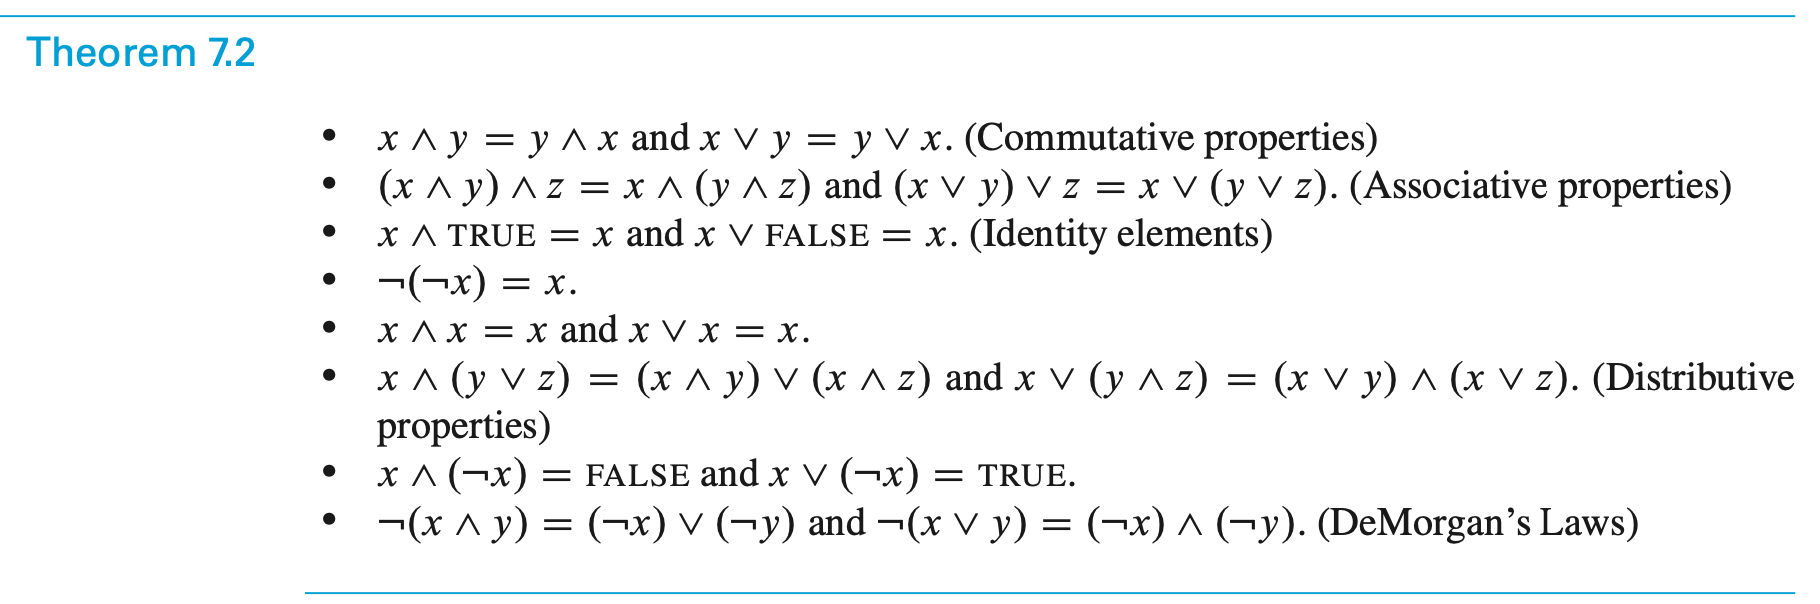
\includegraphics[width=\textwidth]{images/boolean_algebra_properties}
        \caption{Boolean Algebra Properties}
        \label{fig:bap}
\end{figure}
\vfill 

\only<2>{
These properties are proven via truth tables.   You can use them as \alert{shortcuts}.
\vspace{-.5cm}
\hfill 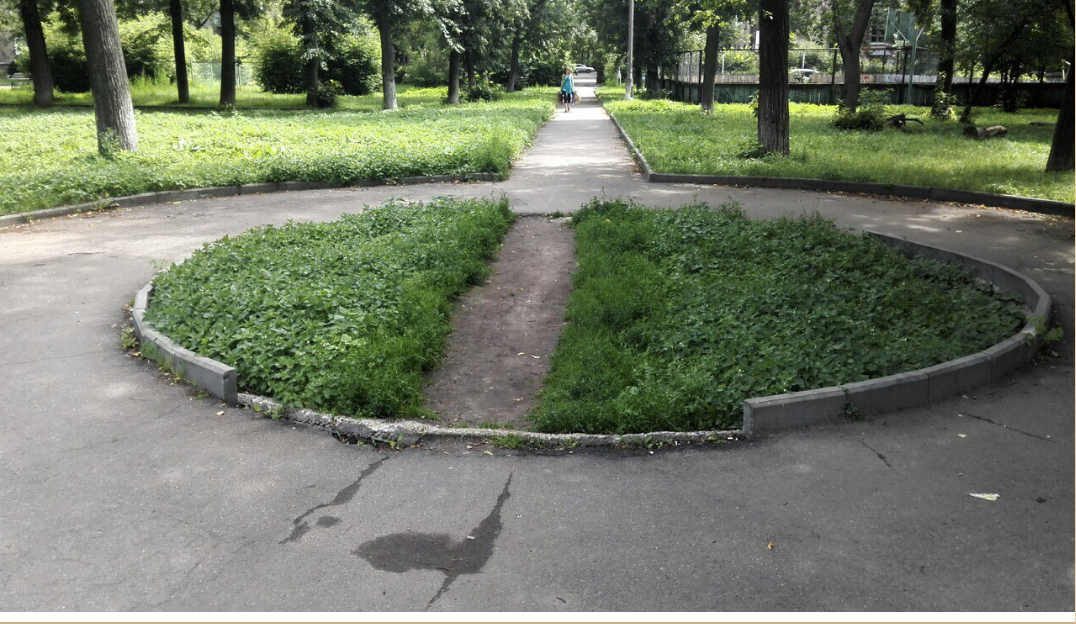
\includegraphics[height=2.5cm]{images/shortcut}.
}

\only<3>{
\begin{center}
{\Huge
$\explaintermbrace{and}{\land} \qquad \explaintermbrace{or}{\lor}$
}
\end{center}
}


\end{frame}

\begin{frame}{Boolean Algebra Properties: Example}
\small 
\begin{myredbox}[title=DeMorgan's Laws]
For propositions $P$ and $Q$:
\[ 1. \quad \lnot (P \land Q) = (\lnot P) \lor (\lnot Q) \qquad \qquad 2. \quad \lnot (P \lor Q) = (\lnot P) \land (\lnot Q)\]
\end{myredbox}

\vfill 

\only<1-2>{\begin{myyellowbox}[title=Poll]
How can we understand/interpret these?
\end{myyellowbox}
}

\vfill 
\pause 
\only<2>{\begin{mygreenbox}[title=Verbalization]
\begin{enumerate}
	\item 	\qq{Not (P and Q)} is the same as \qq{(Not P) or (Not Q).}
	\item \qq{Not (P or Q)} is the same as \qq{(Not P) and (Not Q).}
\end{enumerate}
\end{mygreenbox}}




\only<3>{\begin{mygreenbox}[title=People use these all of the time in conversation!]
\footnotesize
\underline{Law 1}\quad \qq{You can't \red{have your cake} \textbf{and} \blue{eat it too}.}

Means: either you don't \red{have it}, \textbf{or} you don't \blue{eat it}. That is $\lnot(P \land Q) = (\lnot P) \lor (\lnot Q)$.

\vspace{0.5em}
\underline{Law 2}\quad \qq{I don't \red{drink} \textbf{or} \blue{smoke}.}

Nobody hears that as \qq{or}.  Everyone hears
\qq{I don't \red{drink} \textbf{and} I don't \blue{smoke}}. That is, $\lnot(P \lor Q) = (\lnot P) \land (\lnot Q)$, applied without noticing.

%\vspace{0.4em}
%\alert{\textbf{The laws are not new. Only the notation is.}}
\end{mygreenbox}}


%\only<3>{\begin{mygreenbox}[title=Everyday example]
%\footnotesize 
%Suppose $P:$ Paul is at the party. $Q:$ Kunal is at the party.
%
%\underline{Law 1}:
%\begin{enumerate}
%	\item \textbf{Left side}: \qq{It’s not true that Paul and Kunal are both at the party.}
%	\item  \textbf{Right side}: \qq{Either Paul is not at the party, or Kunal is not at the party (or both).}
%\end{enumerate}
%\greencheck Same meaning! If they're not both there, then at least one of them must be absent.
%
%\underline{Law 2}:
%\begin{enumerate}
%	\item \textbf{Left side}: \qq{It’s not true that Paul or Kunal is at the party..}
%	\item  \textbf{Right side}: \qq{Paul is not at the party, and Kunal is not at the party.}
%\end{enumerate}
%\greencheck Again the same. If the party doesn’t have either one, then both must be absent.
%\end{mygreenbox}}



\only<5>{\begin{mygreenbox}[title=Visual intuition]
\begin{center}
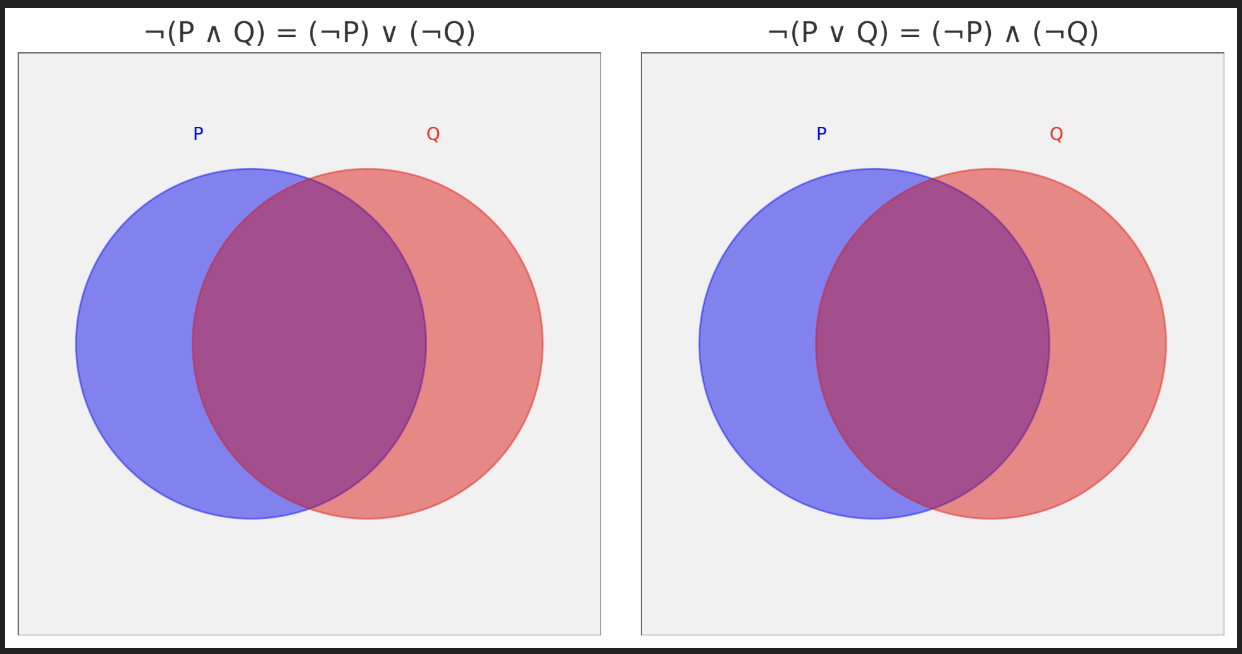
\includegraphics[width=.75\textwidth]{images/demorgan.png}
\end{center}
\footnotesize 
\vspace{-.4cm}
\begin{itemize}
	\item On the left,  $\lnot (P \land Q)$: everything except the overlapping middle part.
	\item On the right,  $\lnot (P \lor Q)$: everything outside both circles.
\end{itemize}

\end{mygreenbox}
}

\end{frame}


\end{document}
